\chapter{Introdução}
Num mundo altamente mecanizado, a força e o torque dentro de todas as grandezas, são as mais comuns. Estas tem um papel significante nos produtos de medição de massa e células de carga usadas na industria e retalho, nos automóveis e nas aeronaves, no aperto de tampas de frascos de medicina e parafusos.\cite{book-9}\\
\\
A massa é uma das grandezas fundamentais, uma propriedade intrínseca de um objeto, na qual se mede pela sua resistência a aceleração.\cite{book-2}
\begin{figure}[H]
	\centering
	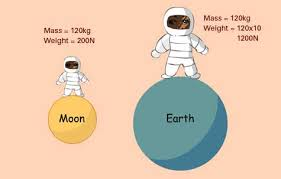
\includegraphics[height=7cm]{./image/PESTA/fisica/mass.jpg}
	\caption{Peso e Massa}
	\label{mass}
\end{figure}
Através da medição do peso, isto é, da força gravitacional exercida num dado objeto, podemos calcular a massa. \cite{book-2}\\
\\
As balanças digitais estão presentes no nosso dia a dia, e tornam-se numa ferramenta indispensável na industria, comercio e laboratórios. Determinar a massa dos objetos facilitou a moeda de troca no comercio, e tornou-se num pilar fundamental da física e seu desenvolvimentos. Existe uma demanda tanto da área comercial como industrial que empurra o desenvolvimento dos sensores para obter melhores resultados quanto a precisão e imunidade de influencias exteriores na medição das grandezas mencionadas.\\
\\
Devido à importância desta grandeza (massa), foi a razão de querer desenvolver uma balança digital para uso domestico usando os meios que estão disponíveis no mercado.
\newpage
\section{Objetivos}
O Objetivo principal deste projeto será fazer uma balança digital economicamente viável, usando os sensores e equipamentos disponíveis no mercado, para ter um produto útil fácil de se replicar.
\\
\\
Escolher o sensor adequado e meios de tratamento da informação e comunicação, será o objeto de estudo. Tendo como foco a utilização de um \textit{Embeded System} utilizando as ferramentas necessárias para o executar.
\\
\\
No final tentar aperfeiçoar, fazer melhorias, alterações e adaptações que possam surgir, de forma a simplificar o progecto e torna-lo mais atraente ao consumidor final.
\newpage
\section{Calendarização}
O segundo semestre teve inicio em 8 de Março, num ambiente de pandemia COVID-19 onde fomos forçados ao ensinamento à distancia, e todo o trabalho teve de ser acompanhado \textit{online} pelos docentes. No entanto tive de organizar as tarefas pretendidas no plano abaixo descrito, para poder fazer a entrega deste trabalho, antes da data limite da época normal 28 de Junho de 2021.
\\
\\
%%%%%%%%%%%%%%%%%%%%%%%%%%%%%%%%%%%%%%%%%%%%%%%%%%%%%%%%%%%%%%%%
\begin{table}[H]
	\caption{Calendarização das tarefas}
	%\begin{sidewaysfigure}
	\begin{ganttchart}[vgrid, hgrid]{1}{20}
		\gantttitle{Março}{5} 
		\gantttitle{Abril}{5}
		\gantttitle{Maio}{5}
		\gantttitle{Juno}{5}\\
		\gantttitlelist{1,...,20}{1}\\
		%First Group
		\ganttgroup{Requisitos}{2}{10} \\
		\ganttbar{Material}{3}{5} \\
		\ganttbar{\textit{Template} LaTeX}{5}{10} \\
		\ganttbar{\textbf{IDE} \textit{Template}}{3}{10}\\
		%\ganttlink{elem0}{elem1}
		%\ganttlink{elem1}{elem2}
		%\ganttlink{elem2}{elem3}
		%\ganttmilestone{Milestone 1}{11}
		%Second Group
		\ganttgroup{Projecto}{3}{20} \\
		\ganttbar{Kit Desenvolvimento}{3}{4} \\
		\ganttbar{Montagen Mesa Sensor}{5}{7} \\%5 7
		\ganttbar{HX711 comunicação}{4}{10} \\%4 8
		\ganttbar{Programção e Ensaio}{4}{20}\\
		%\ganttlink{elem4}{elem5}
		%\ganttlink{elem5}{elem6}
		%\ganttlink{elem6}{elem7}
		%\ganttmilestone{Milestone 1}{11}
		%Third Group
		\ganttgroup{Relatório}{9}{20} \\
		\ganttbar{Literartura}{8}{12} \\
		\ganttbar{Analise Documentação}{9}{12} \\
		\ganttbar{Validação}{10}{12} \\
		\ganttbar{Execução}{10}{20}
		%\ganttlink{elem8}{elem9}
		%\ganttlink{elem9}{elem10}
		%\ganttlink{elem10}{elem11}
		%\ganttmilestone{Milestone 1}{11}
	\end{ganttchart}
	\label{gantt}
%\end{sidewaysfigure}
\end{table}
\newpage
\section{Organização do Relatório}
No capítulo 1 é feita uma contextualização do trabalho realizado e do seu propósito face às necessidades do mundo atual.\\
\\
No capítulo 2 vai ser descrito uma breve historia da evolução das balanças, e depois um estudo da balança digital.
%%%%%%%%%%%%%%%%%%%%%%%%%%%%%%%%%%%%%%%%%%%%%%%%%%%%%%%%%%%%%%%%
\chapter{História da Balança}
%%%%%%%%%%%%%%%%%%%%%%%%%%%%%%%%%%%%%%%%%%%%%%%%%%%%%%%%%%%%%%%%
As balanças foram criadas por necessidade durante o desenvolvimento do comercio na antiguidade. Os produtos que não recorriam a contagem por unidades, tais como objetos irregulares (por exemplo o ouro) tinha de se quantificar o seu valor, e a forma de medir a sua massa tornou-se numa variável de medição para a troca de bens.
\\
\\
A relíquia mais antiga de uma balança de medir massa, foi descoberto na vila de \textit{Indus River}, perto do conhecido por hoje de Pakistão, e estima-se ser por volta de \textcolor{blue}{2000} A.C.
\\
Estas primeiras balanças eram alavancas em equilíbrio $[ \; F_{1} \times b_{1c} = F_{2} \times b_{2c} \; ]$, onde nos extremos eram colocados cestos e se colocava os pesos, este estava centrado no seu centro de massa, assim se os pesos nos dois cestos fossem iguais, a alavanca ficava em equilíbrio (na horizontal), tornando-se nessa altura num sistema de cmparação, com recursos a pesos fixos estabelecidos como norma e designados de (\textbf{contra-pesos}).
\\
\begin{minipage}[!b]{0.45\linewidth}
	\begin{figure}[H]
		\centering
		\includegraphics[height=7cm]{./image/PESTA/general/balanca_1.jpg}
		\caption{Balança medieval}
		\label{balanca_1}
	\end{figure}
\end{minipage}
\hspace{2.2cm}
\begin{minipage}[!b]{0.45\linewidth}
	\begin{figure}[H]
		\centering
		\includegraphics[height=7cm]{./image/PESTA/general/balanca_4.jpg}
		\caption{Balança}
		%\caption{Balança moderna \cite{book-7}}
		\label{balanca_4}
	\end{figure}
\end{minipage}
\newline
\newline
\newline
Este sistema pode ter uma boa precisão, mas também pode se facilmente ser adulterado.
\\
\\
Os métodos de medir a massa de objetos não conheceu nenhumas melhorias tecnológicas relevantes até a era industrial. Só nos fins do século \textcolor{blue}{\textit{XVIII}} é que o meio de medir a massa de objetos não dependia de \textbf{contra-pesos}. As balanças por molas foram inventado por  por volta de \textcolor{blue}{1770} em Inglaterra por \textbf{\textit{Richard Salter}}, um fabricante de balanças.
\\
\begin{figure}[H]
	\centering
	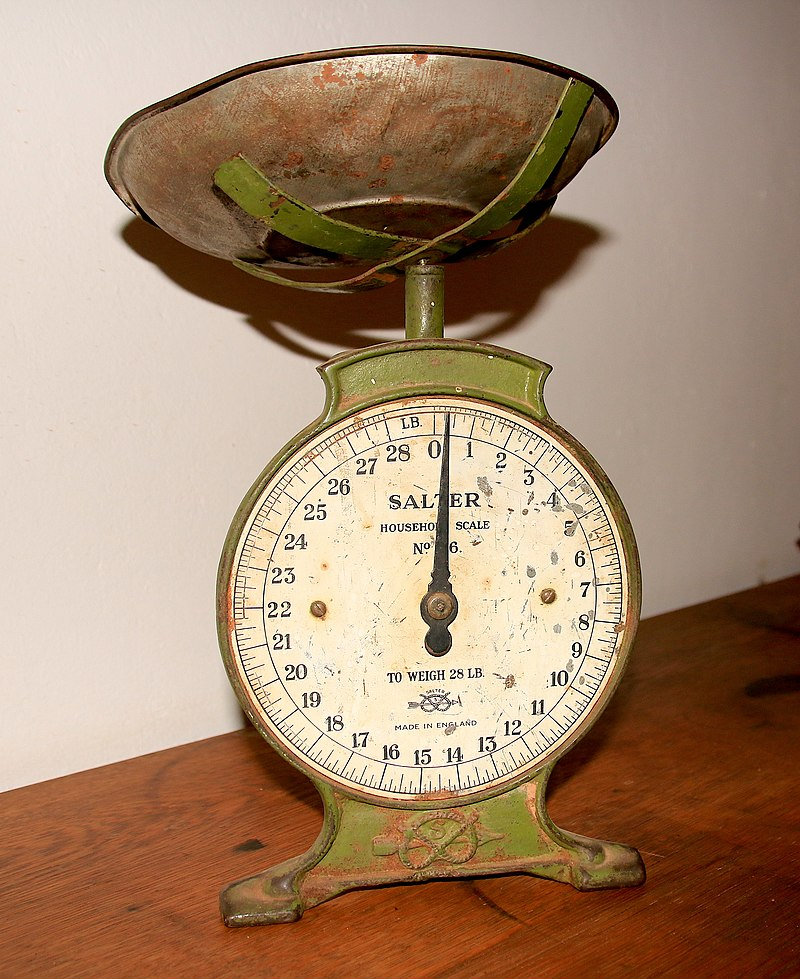
\includegraphics[height=7cm]{./image/PESTA/general/Weigh_Scale_Salter_1.jpg}
	\caption{Balança de Salter}
	\url{https://en.wikipedia.org/wiki/Salter_Housewares}
	\label{Weigh_Scale_Salter_1}
\end{figure}
A balança por mola, como o nome implica, mede a pressão (ou sua tensão) exercido sobre a mola para determinar a massa do objeto. Este tipo de balanças ainda são muito comum nos dias de hoje por serem bastante económicas de fabricar, mas não tem tanta precisão como as eletrónicas desenvolvidas e aperfeiçoadas durante o século \textcolor{blue}{\textit{XX}}.
\newline
\newline
\begin{minipage}[!b]{\linewidth}
	\begin{figure}[H]
		\captionsetup{justification=raggedright,singlelinecheck=false}
		\flushleft
		\includegraphics[height=7cm]{./image/PESTA/general/Public_Body_Scales_1.jpg}
		\hspace{.8cm}
		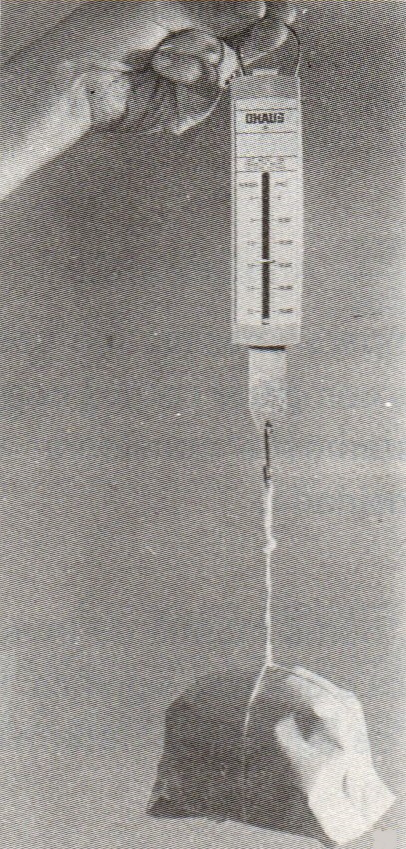
\includegraphics[height=7cm]{./image/PESTA/general/Balanca_Mola_1.jpg}
		\caption{Balanças de Mola}
		\label{Balanca_Mola_1}
	\end{figure}
\end{minipage}
\newpage
As balanças eletrónicas mais modernas, utilizam resistências elétricas instaladas sobre materiais flexíveis por onde passa uma corrente elétrica, na qual é possível detetar a variação de condutividade das resistências. Esta variação é proporcional à pressão exercida sobre esse material, podendo dai obter-se o peso dos objetos.
\\
\begin{figure}[H]
	\centering
	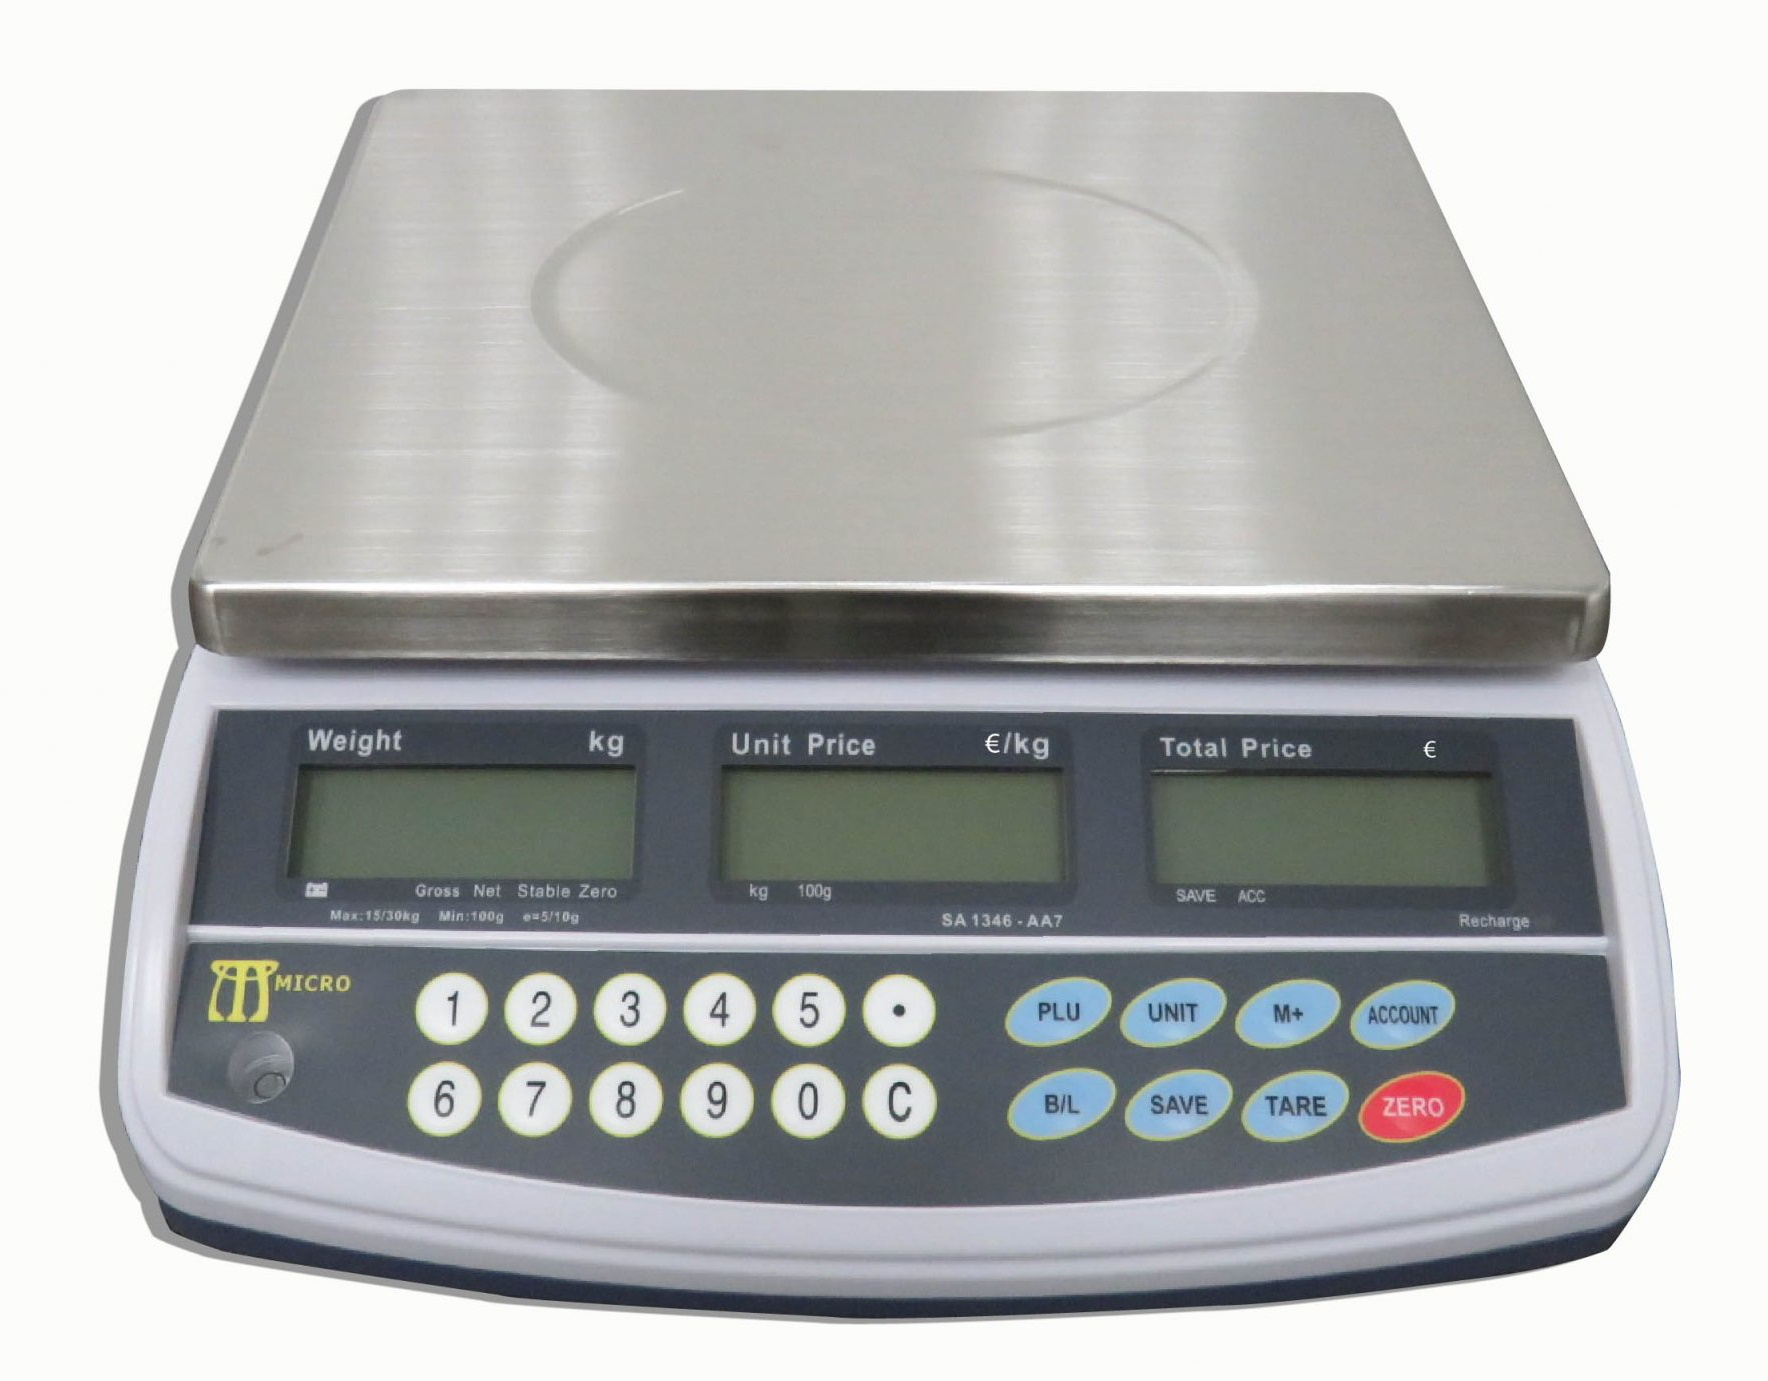
\includegraphics[height=7cm]{./image/PESTA/general/Scale_1.jpg}
	\caption{Balança eletrónica}
	\label{Scale_1}
\end{figure}
O que vai ser utilizado no projeto vai ser um \textbf{célula de carga}, que segue o principio acima mencionado. Estas células tem quatro sensores \textit{\textbf{strain gauges}} ligadas em ponte \textit{wheatstone}, que vão detetar a distorção (pressão) do material, ou seja, da célula de carga e gerar um sinal em tensão proporcional a força exercida quando alimentada. Seque o mesmo principio de uma mola.
\begin{equation}
	\label{eq:Hooke}
	K = \frac{\Delta l}{F}
\end{equation}
Outros tipos de células de peso tais como as pneumáticas e hidráulicas que convertem a pressão num sinal elétrico que é proporcional a força nela exercida.
\begin{equation}
	\label{eq:Preasure}
	P = \frac{F}{A}
\end{equation}
As células de peso capacitivas são outro exemplo de como obter um sinal proporcional a força imposta como carga, neste caso é medido sua capacidade pelo afastamento ou aproximação dos pratos dos elétrodos.
\begin{equation}
	\label{eq:Capacity}
	C = \varepsilon_{0} \; \varepsilon_{r} \; \frac{A}{d}
\end{equation}
Também existe células que utilizam o principio de ressonância e desfasamento de fase e efeito \textit{doppler} para determinar a pressão ou distorção das células de peso e consequente uma medição.
\\
\\
Pode-se dizer que em todos os casos determina-se a força resultante através do deslocamento no espaço.
%%%%%%%%%%%%%%%%%%%%%%%%%%%%%%%%%%%%%%%%%%%%%%%%%%%%%%%%%%%%%%%%
\begin{comment}
Measurement devices need to be robust to withstand changing environmental influences such as temperature, vibration, and humidity, and they must also provide reliable measurement over long periods of time. Mechanical interfacing of the devices can be difficult and can influence final measurement. The forces and torques may change rapidly, and so the devices must have adequate frequency and transient responses.\\
There are several methods to measure forces and torques. Often, the force to be measured is converted into a change in length of a spring element. The change in dimensions is subsequently measured by a sensor, for example, a piezoresistive, a capacitive or a resonant sensor.\\
It is not so surprising, therefore, that most force and torque measurement devices utilize the long and well-established resistance strain gauge technology.\\
Unfortunately, the metallic resistance strain gauge is relatively insensitive such that in use it is normal to obtain only several millivolts of analog voltage before amplifi-
cation, and the gauges must not be significantly overstrained. The rangeability and overloading capabilities are seriously restricted. Also, the gauges consume relatively high electrical power (e.g., 250 mW).\\
In general, measurement instrumentation now needs smaller sensing devices of lower power consumption and with greater rangeability and overload capabilities.\\
Greater compatibility with digital microelectronics is highly desirable. Noncontact and wireless operation is sometimes needed, and in some cases batteryless devices
are desirable. Production of measurement devices using metallic resistance strain gauges can be relatively labor intensive and skilled, and may require relatively ineffi-cient calibration procedures.\\
In recent years some instrument manufacturers of force and torque measure-ment devices have moved away from using resistance strain gauges. Already, one leading manufacturer of weighing machines for retail and industrial applications
now uses metallic and quartz resonant tuning fork technologies, and smaller compa-nies have established niche markets using surface acoustic wave (SAW) technology, optical technology, and magnetoelastic technology.\\
Further commercial developments are taking place to enhance device manufacturability and improve device sensitivity and robustness in operation. Measurement on stiffer structures at much lower strain levels is now possible. The worldwide sen-
sor research base is very active in exploring MEMS for sensing force and torque, and the rest of this chapter will review the current situation and future prospects.\\
\\
The market pull provided by the automotive industry—for example,
for manifold air pressure sensors—has led to the development of successful devices and technologies that have benefited a wide range of other pressure sensing applica-tions.
\end{comment}